\lecture{1}{25. August 2025}{Introduction to Fluid Mechanics}

\section{Fundamental Concepts}

\subsection{Fluid as a Continuum}
Fluids are normally experienced as being continuous or ``smooth'' when percieved in the macroscopic world. If one looks at a fluid microscopically one would start to see that the fluid is not continuous at all but instead composed of distinct particles. We wish to determine the minimum volume, $\partial V'$ that a point $C$ must be such that we can talk about the fluid being continous at this point. In other words, under what circumstances can a fluid be treated as a continuum, for which, by definition, properties vary smoothly over all points. 

We define the mass $\partial m$ as the instantaneous number of molecules in $\partial V $ and the mass of each of these molecules. The average density inside volume $\partial V $ is hence given by $\rho = \frac{\partial m }{\partial V }$. It is important to note that this necessarily is an \textit{average value} as the number of molecules in $\partial V $ and hence the density fluctuates. Due to the law of large numbers one will experience that for very small volume the density will fluctuate greatly over time, however at a certain volume $\partial V' $, the density becomes stable and will not fluctuate greatly over time. For $\partial V = \qty{0,001}{mm^3}  $ (about the size of a grain of sand) there will already be an average of \num{2,5e13} molecules present. Hence a liquid can be treated as a continuous medium as long as we consider a ``point'' to be no smaller than about this size -- at least this is sufficiently precise for most engineering appplications.

This continuum hypothesis is an integral part of fluid mechanics. It is valid when treating the behaviour of fluids under normal conditions and only breaks down when the mean free path of the molecules becomes the same order of magnitude as the smallest characteristic dimension of the problem. 

As a consequence of the continuum assumption, each property of the fluid is assumed to have a definite value at each point in space. I.e. density, temperature, velocity, and so on are each continuous functions of both position and time. We now have a definition of the density at a point:
\[ 
\rho \equiv \lim_{\partial V \to \partial V'  } \frac{\partial m }{\partial V }
.\]
As point $C$ was chosen arbitrarily the density at any other point in the liquid can be determined in the same manner. If one measures this simultaneously for all points in the fluid, an expression for the density distribution as a function of the space coordinates $\rho = \rho(x,y,z)$ can be found.

The density at a specific point may also vary with time. Therefore the complete representation of density, the so-called \textit{field representation}, can be written as:
\begin{equation} \label{eq:dens}
\rho = \rho(x,y,z,t)
\end{equation}
As density is a scalar quantity the field given by \autoref{eq:dens} is a scalar field. 

The density can also be expressed as the specific gravity, i.e. the weith compared to the maximum density of water, $\rho_{\mathrm{H}_2 \mathrm{O}} = \qty{1000}{\frac{kg}{m^3}} \text{ at } \qty{4}{\celsius} $. Thus the specific gravity of a substance can be found as:
\[ 
\mathrm{SG} = \frac{\rho}{\rho_{\mathrm{H}_2 \mathrm{O}}}
.\]

Another useful property is the \textit{specific weight}, $\gamma$, of a substance. It is defined as the weight of a substance per unit volume, i.e.:
\[ 
\gamma = \frac{mg}{V} \implies \gamma = \rho g
.\]

\subsection{Velocity field}
A very important property defined by a field is the velocity field, given by:
\begin{equation} \label{eq:velo}
  \textbf{V} = \textbf{V}(x, y, z, t)
\end{equation}
As velocity is a vector quantity, the field given in \autoref{eq:velo} is a vector field.

The velocity vector, $\textbf{V}$, can also be written in terms of its scalar components. Denoting the components in the $x$-, $y$-, and $z$-directions by $u$, $v$, and $w$, respectively we get:
\[ 
\textbf{V} = u \hat{i} + v \hat{j} + w \hat{k}
.\]
Here, each component, $u$, $v$, and $w$, will generally be functions of $x$, $y$, $z$ and $t$.

We also need to be make sure to remember that $\textbf{V}(x, y, z, t)$ represents the velocity of a fluid particle passing through the point $(x,y,z)$ at time $t$. Therefore $\textbf{V}(x,y,z,t)$ should be thought of as the velocity field of the entire fluid and not of an individual particle.

If properties at every point in a flow field are constant with respect to time, the flow is termed \textit{steady}. This is defined mathematically as:
\[ 
\frac{\partial \eta}{\partial t} = 0
.\]
Where $\eta$ is any fluid property. Hence, for steady flow:
\[ 
\frac{\partial \rho}{\partial t} = 0 \text{ or } \rho = \rho(x,y,z)
\]
and
\[ 
\frac{\partial \textbf{V}}{\partial t} = 0 \text{ or } \textbf{V} = \textbf{V}(x,y,z)
.\]
As such any property may vary from point to point in the field but remain constant with time at every point for steady flow. 


\subsection{One-, Two-, and Three-Dimensional flows}
A flow is either one-, two-, or three-dimensional depending on the amount of spatial coordinates required to specify the velocity field. \autoref{eq:velo} shows that the velocity field in some cases is a function of three spatial coordinates and time -- in this case it is a three-dimensional flow.

Almost all flows are three-dimensional in nature -- however, analysis based on fewer dimensions is often sufficient. The complexity of analysis increases sharply as more dimensions are added, and oftentimes in engineering a one-dimensional analysis is sufficient. 

To not break the continuum assumption all fluids must have zero velocity at any solid surface, e.g. the inner side of a pipe. Due to this all flow in pipes is inherently three-dimensional. To simplify the analysis one often uses the notion of \textit{uniform flow} at a given cross-section. In a flow that is uniform at a given cross-section, the velocity is constant across any section normal to the flow as shown in \textbf{\autoref{fig:f2_3}}. Under this assumption, the flow simplifies to be simply a function of $x$ alone. The term \textit{uniform flow field} is used to describe a flow in which the velocity is constant throughout the entire field.

\begin{figure} [ht]
  \centering
  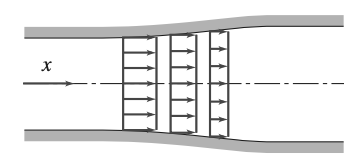
\includegraphics[width=0.5\linewidth]{./figures/f2_3.png}
  \caption{\textit{Uniform flow} at a given cross-section.}
  \label{fig:f2_3}
\end{figure}

\begin{definition}[Uniform flow at a cross section]
  An assumption that states that a fluid has the same velocity everywhere in a given cross section as shown on \textbf{\autoref{fig:f2_3}}. This actually breaks the continuum hypothesis but it makes a lot of calculations easier.
\end{definition}

\begin{definition}[Uniform flow field]
  A flow field where the velocity is constant everywhere throughout the flow field.
\end{definition}


\subsection{Timelines, Pathlines, Streaklines, and Streamlines}
Wind tunnels have traditionally often utilized to visualize flow fields. In modern times the advent of computer simulations has meant that these have become much more prevalent recently. A few different terms must be defined for proper understanding of these.

\begin{definition}[Timeline]
  A \textit{timeline} is produced by marking adjacent fluid particles in a flow field at a given instant. Subsequent observation of the timeline can give insights into the flow field.
\end{definition}

\begin{definition}[Pathline]
  A \textit{pathline} is the trajectory traced out by a moving fluid particle. These can be visualized by marking a fluid particle at a given instant, e.g. with dye or smoke, and then tracing the path of this particle as it moves through the field.
\end{definition}

\begin{definition}[Streakline]
  A \textit{streakline} is the line traced out by marking the fluid particles at a fixed point in space, e.g. with smoke or dye. This is therefore a way to see how fluid particles that passed through a specific point behave afterwards.
\end{definition}

\begin{definition}[Streamlines]
  A \textit{streamline} are lines drawn in a flow field such that at any given instant they are tangent to the velocity vector at every point in the flow. This means there can be no flow across a streamline. These are the most commonly used visualization technique
\end{definition}

We can use the velocity field to derive the shapes of streaklines, pathlines and streamlines. As the streamlines are parallel to the velocity vector, for a two dimensional flow field, we can write:
\begin{equation} \label{eq:stre}
  \frac{\mathrm{d}y}{\mathrm{d}x} \bigg|_{\text{streamline}} = \frac{v(x,y)}{u(x,y)}
\end{equation}
Note that these are obtained at a given instant in time. If the flow is unsteady, time $t$ is held constant in \textbf{\autoref{eq:stre}}. Solution of the equation gives $y = y(x)$, with an undetermined integration constant, the value of which depends on the particular streamline.

For pathlines, we let $x = x_p(t)$ and $y = y_p(t)$ where $x_p(t)$ and $y_p(t)$ are the instantaneous coordinates of a specific particle. In this case we get
\begin{equation} \label{eq:path}
  \frac{\mathrm{d}x}{\mathrm{d}t} \bigg_{\text{particle}} = u(x,y,t) \qquad \frac{\mathrm{d}y}{\mathrm{d}t} \bigg_{\text{particle}} = v(x,y,t)
\end{equation}
The simultaneous solution of these equations gives the path of a particle in parametric form, $x_p(t), y_p(t)$.

For streaklines, the first step is to compute the pathline of a particle with \autoref{eq:path} that was released from the streak source at $x_0$, $y_0$ at time $t_0$, in the form
\[ 
x_{\text{particle}} (t) = x(t, x_0, y_0, t_0) \qquad y_{\text{particle}}(t) = y(t, x_0, y_0, t_0)
.\]
Then now, instead of interpreting this as the position of a particle over time, we instead write the equations as:
\begin{equation}\label{eq:streak}
  x_{\text{streakline}} \left( t_0 \right) = x \left( t, x_0, y_0, t_0 \right) \qquad y_{\text{streakline}} \left( t_0 \right) = y \left( t, x_0, y_0, t_0 \right)
\end{equation}
\autoref{eq:streak} gives the line generated (by time $t$) from a streak source placed at $(x_0, y_0)$. In these equations $t_0$ is varied from $0$ to $t$ to show the \textit{instantaneous} positions of all particles released up to time $t$. 

\subsection{Stress Field}
To understand the behaviour of fluids one must first understand the nature of the forces that act upon fluid particles. A fluid particle can experience either:
\begin{itemize}
  \item \textit{Surface forces}, e.g. pressure or friction, that are generated due to contact with other particles or surfaces
  \item \textit{Body forces}, e.g. gravity and electromagnetic, that are experienced throughout the particle.
\end{itemize}

Surface forces on a fluid particle leads to \textit{stresses}. Stress is an important concept when describing how forces acting on the boundaries of a medium are transmitted throughout the medium. 

We consider the surface of a particle in contact with other fluid particles and the contact force being generated between these. Let $\delta \textbf{A}$ be a portion of the surface at some point $C$. The orientation of $\delta \textbf{A}$ is given by the unit vector $\hat{n}$, which is perpendicular to the surface as seen in \textbf{\autoref{fig:f2_6}}.

The force, $\delta \textbf{F}$, acting on the surface portion $\delta \textbf{A}$ may be split into two components -- a \textit{normal stress} $\sigma_n$ normal to the surface and a \textit{shear stress} $\tau_n$ tangential to the surface, defined as:
\begin{align*}
  \sigma_n &= \lim_{\sigma A_n \to 0} \frac{\delta F_n}{\delta A_n} \\
  \tau_n &= \lim_{\delta A_n \to 0} \frac{\delta F_t}{\delta A_n}
.\end{align*}

The subscript $n$ on the stress is a reminder that the stresses are associated with the surface portion $\delta \textbf{A}$ through $C$, which has an outward normal in the $\hat{n}$ direction. 

\begin{figure} [ht]
  \centering
  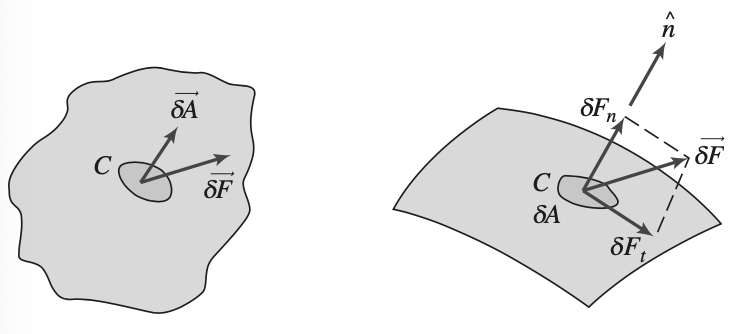
\includegraphics[width=0.5\linewidth]{./figures/f2_6.png}
  \caption{Stress in a continuum.}
  \label{fig:f2_6}
\end{figure}

We consider the stress on the element $\delta A_x$ whose normal is in the $+x$-direction. We can then split the force acting upon this point $\delta \textbf{F}$ into components along each coordinate direction. By dividing the magnitude of each force component by the area $\delta A_x$ and taking the limit as $\delta A_x$ approaches zero we define three stress components as:
\begin{align*}
  \sigma_{ x x} &= \lim_{\delta A_x \to 0} \frac{\delta F_x}{\delta A_x} \\
  \tau_{xy} &= \lim_{\delta A_x \to 0} \frac{\delta F_y}{\delta A_x} \\
  \tau_{xz} &= \lim_{\delta A_x \to 0} \frac{\delta F_z}{\delta A_x}
.\end{align*}
This is also shown graphically in \textbf{\autoref{fig:f2_7}}.

\begin{figure} [ht]
  \centering
  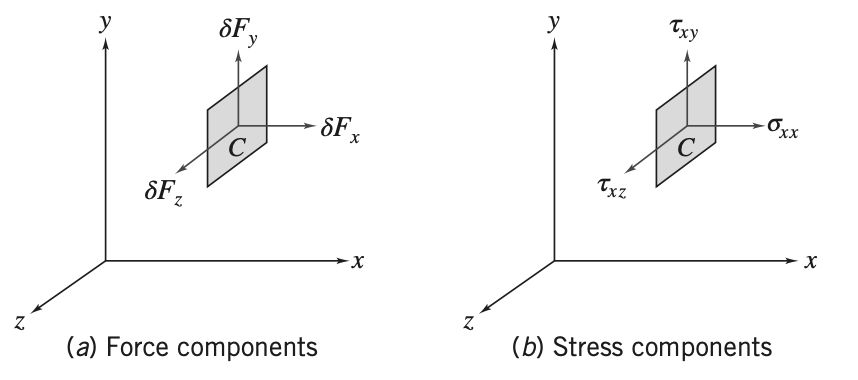
\includegraphics[width=0.5\linewidth]{./figures/f2_7.png}
  \caption{Force and stresses at surface element $\delta A_x$}
  \label{fig:f2_7}
\end{figure}

Here the first subscript ($x$) indicates the \textit{plane} on which the stress acts, in this case a surface perpendicular to the $x$-axis. The second direction indicates the \textit{direction} in which the stress acts. I.e. consideration of the element $\delta A_y$ would lead to the stresses $\sigma_{yy}$, $\tau_{yx}$ and $\tau_{yz}$ and similarly for $\delta A_{z}$. 

As the coordinate system was chosen arbitrarily it is easily realized that one can define an infinite amount of stresses through a point $C$ depending on how the axes are placed. Luckily, the state of stress at any point is completely described by the stresses acting in any three mutually perpendicular planes through the point. Therefore the stress at a point is specified by the nine components:
\[ 
\begin{bmatrix}
\sigma_{x x} & \tau_{xy} & \tau_{xz}\\
\tau_{yx} & \sigma_{yy} & \tau_{yz}\\
\tau_{z x} & \tau_{zy} & \sigma_{zz}\\
\end{bmatrix}
.\]
Planes are normally named for the direction in which their normal vector is pointing. Also we normally define a stress component to be positive when the stress component and the plane on which it acts are either both positive 
